\begin{figure}
\begin{tabular}{@{}c@{}c@{}}
\begin{subfigure}[b]{0.5\textwidth}
\begin{center}
\begin{footnotesize}
\renewcommand{\arraystretch}{1.5}
\begin{tabular}{ll}
\toprule
\multicolumn{2}{c}{\bf Points-to Invariants} \\
\midrule
$\circled{\footnotesize J1} \  \cv{p} \pointsTo{} \{ \mlrf{\cpc{4}} \}$ & $\circled{\footnotesize J2} \  \mlrf{\cpc{4}} \pointsTo{} \{ \mlrs{\cpc{4}} \}$ \\
$\circled{\footnotesize J3} \  \cv{l} \pointsTo{} \{ \mlrs{\cpc{4}} \}$ & $\circled{\footnotesize J4} \  \mlrs{\cpc{4}} \pointsTo{} \{ \mlrs{\cpc{4}}, \heapr{} \}$ \\
$\circled{\footnotesize J5} \  \cv{i} \pointsTo{} \emptyset$            & $\circled{\footnotesize J6} \  \heapr{} \pointsTo{} \{ \mlrs{\cpc{4}}, \heapr{} \}$ \\
\bottomrule
\end{tabular}
\end{footnotesize}
\end{center}
\caption{\label{fig:clistdeconspointstoinvs}Points-to invariants at \cpc{5} of \cref{fig:llAllocCIR}}
\end{subfigure}%
&
\begin{subfigure}[b]{0.5\textwidth}
\begin{center}
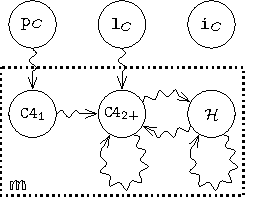
\includegraphics[scale=1]{chapters/figures/figClistDeconsCfgPointstoGraph.pdf}
\end{center}
\caption{\label{fig:clistdeconspointstograph}Points-to graph at \cpc{5} of \cref{fig:llAllocCIR}}
\end{subfigure}%
\\
\end{tabular}
\caption{\label{fig:clistdeconspointstoinvsandgraph}Points-to invariants at \cpc{5} of \cprog{} in \cref{fig:llAllocCIR}.
\Cref{fig:clistdeconspointstograph} shows the graphical representation of the relations in \cref{fig:clistdeconspointstoinvs}.
Each node represents a \cprog{} pseudo-register or a memory region in \mem{}. An edge $A \rightarrow R$ represents the condition
that $A$ (or objects in $A$ in case of a memory region) may point to the memory region $R$.}
\end{figure}